\documentclass[12pt]{article}
\usepackage{graphicx}
\usepackage[a4paper, margin=1in]{geometry}
\usepackage{amsmath}
\usepackage[utf8]{inputenc}
\usepackage{listings}
\usepackage{xcolor}

\usepackage{amsfonts}
\usepackage{amssymb}
\usepackage{geometry}
\usepackage{titlesec}
\usepackage{fancyhdr}
\usepackage{lipsum}


\lstdefinestyle{mystyle}{
    backgroundcolor=\color{white},
    commentstyle=\color{codegreen},
    keywordstyle=\color{magenta},
    numberstyle=\tiny\color{codegray},
    stringstyle=\color{codepurple},
    basicstyle=\ttfamily\footnotesize,
    breakatwhitespace=false,
    breaklines=true,
    captionpos=b,
    keepspaces=true,
    numbers=left,
    numbersep=5pt,
    showspaces=false,
    showstringspaces=false,
    showtabs=false,
    tabsize=2
}

\lstset{style=mystyle}

\definecolor{codegreen}{rgb}{0,0.6,0}
\definecolor{codegray}{rgb}{0.5,0.5,0.5}
\definecolor{codepurple}{rgb}{0.58,0,0.82}

% Configuración de página
\geometry{a4paper, margin=1in}
\pagestyle{fancy}
\fancyhf{}
\rhead{Eidan Owen Plata Salinas}
\lhead{Implementacion K-Folds}
\cfoot{\thepage}

% Títulos
\titleformat{\section}[block]{\normalfont\Large\bfseries}{\thesection}{1em}{}
\titlespacing*{\section}{0pt}{\baselineskip}{\baselineskip}

% Metadatos
\title{Implementacion K-Folds}
\author{Eidan Owen Plata Salinas}
\date{\today}


\title{Implementacion K-Folds}
\author{Plata Salinas Eidan Owen}
\date{\today}

\begin{document}
\maketitle
\pagebreak



\section*{Explicacion}
A continuación, se describe el código Python que implementa k-folds. De modo que va comparando mejor modelo.
\vspace{1cm}


\subsection*{Funcion \texttt{CargarDatos}}



\vspace{1cm}

\begin{lstlisting}[language=Python]


def cargar_datos(ruta_csv):
	data = pd.read_csv(ruta_csv, header=None)
	X = data.iloc[:, :-1].values
	y = data.iloc[:, -1].values
	return X, y


\end{lstlisting}
\vspace{1cm}

Esta función se encarga de leer un archivo CSV sin una fila de encabezado (asumiendo que la primera fila ya contiene datos). Luego, separa los datos en características (X) y etiquetas (y) y los devuelve.

\vspace{1cm}

\subsection*{Funcion \texttt{kFoldCrossValidation}}
\vspace{1cm}

\begin{lstlisting}[language=Python]

def k_fold_cross_validation(X, y, k, modelo):
	fold_size = len(X) // k
	indices = np.arange(len(X))
	np.random.shuffle(indices)
	scores = []
	
	for fold in range(k):
	test_indices = indices[fold * fold_size : (fold + 1) * fold_size]
	train_indices = np.setdiff1d(indices, test_indices)
	
	
	X_train, X_test = X[train_indices], X[test_indices]
	y_train, y_test = y[train_indices], y[test_indices]
	
	
	modelo_clonado = clone(modelo)
	modelo_clonado.fit(X_train, y_train)
	
	
	y_pred = modelo_clonado.predict(X_test)
	score = accuracy_score(y_test, y_pred)
	scores.append(score)
	
	return scores

\end{lstlisting}
\vspace{1cm}

Esta función implementa la validación cruzada k-fold manualmente. Divide los datos en k subconjuntos y realiza k iteraciones de entrenamiento y validación, utilizando un subconjunto diferente como conjunto de prueba en cada iteración y el resto como conjunto de entrenamiento.

Dentro del bucle para cada fold, se clona el modelo proporcionado para evitar la contaminación entre los pliegues y se entrena y evalúa el modelo clonado. Después de las predicciones, se calcula la precisión y se guarda en una lista de scores.

\vspace{1cm}

\subsection*{Función \texttt{evaluarConKfoldManual}}
\vspace{1cm}

\begin{lstlisting}[language=Python]

def evaluar_con_kfold_manual(X, y, k=5):
	modelos = {
		'KNN': Pipeline([('scaler', StandardScaler()), ('classifier', KNeighborsClassifier(n_neighbors=5))]),
		'Regresion Logistica': Pipeline([('scaler', StandardScaler()), ('classifier', LogisticRegression(random_state=42))]),
		'SVM': Pipeline([('scaler', StandardScaler()), ('classifier', SVC(kernel='linear', random_state=42))]),
		'Bayesiano': Pipeline([('scaler', StandardScaler()), ('classifier', GaussianNB())])
	}
	
	resultados = dict()

	for nombre, modelo in modelos.items():
	scores = k_fold_cross_validation(X, y, k, modelo)
	resultados[nombre] = scores
	print(f"{nombre}: {np.mean(scores)} (+/- {np.std(scores)})")
	mejor_modelo = max(resultados, key=lambda nombre: np.mean(resultados[nombre]))
	print(f"\nEl mejor modelo es {mejor_modelo} con una precision de {np.mean(resultados[mejor_modelo])}.")

\end{lstlisting}
\vspace{1cm}

Esta función crea un diccionario de modelos de aprendizaje automático, cada uno envuelto en un Pipeline que primero escala los datos y luego aplica el clasificador. Para cada modelo, utiliza la función k\_fold\_cross\_validation para evaluar su rendimiento utilizando la validación cruzada k-fold y luego imprime el rendimiento promedio y la desviación estándar de las puntuaciones de precisión.

\vspace{1cm}

\subsection*{Función \texttt{main}}
\vspace{1cm}

\begin{lstlisting}[language=Python]

def main(ruta_csv):
	X, y = cargar_datos(ruta_csv)
	evaluar_con_kfold_manual(X, y)

\end{lstlisting}
\vspace{1cm}

La función main es el punto de entrada para ejecutar el proceso de evaluación de modelos cuando se ejecuta el script como un programa principal. Carga los datos y llama a la función evaluar\_con\_kfold\_manual.

\vspace{1cm}



\clearpage
\section*{Conclusión}

A través de la función k\_fold\_cross\_validation, he desarrollado en cómo la técnica k-fold divide los datos en partes iguales para entrenar y probar modelos de forma más robusta y confiable. Este enfoque me ha permitido entender mejor la importancia de evaluar el rendimiento del modelo más allá de una simple partición de entrenamiento y prueba, reduciendo la variabilidad y proporcionando una estimación más precisa de cómo el modelo podría desempeñarse en datos no vistos.

Al trabajar con diferentes modelos de clasificación dentro de un pipeline de scikit-learn, incluyendo KNN, regresión logística, SVM y Naive Bayes, he visto cómo el preprocesamiento de datos, como la estandarización, es crucial para algunos algoritmos, especialmente aquellos que son sensibles a la escala de las características. Además, la modularidad y la facilidad de uso de scikit-learn me permitieron intercambiar y evaluar modelos de forma sencilla y directa.

Construir la función evaluar\_con\_kfold\_manual, fue ùtil no solo pude comparar los modelos en términos de precisión media, sino que también pude apreciar las diferencias en la variabilidad de su rendimiento a través de la desviación estándar de las precisiones. Esto me ha dado una visión más completa para determinar cuál es el modelo más adecuado.

A continuacion los resultados.
\vspace{1cm}\vspace{1cm}
\begin{figure}[h] % Coloca la imagen aquí (h significa aquí)
    \centering
    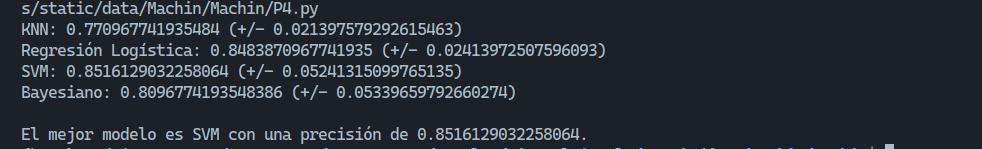
\includegraphics[width=0.9\textwidth]{1.jpg} % Especifica el nombre de la imagen y su ancho relativo al ancho del texto
    \caption{Puntajes del dataset} % Agrega una descripción o título a la imagen
    \label{fig:1} % Etiqueta para referenciar la figura en el texto
\end{figure}
\vspace{1cm}\vspace{1cm}



\clearpage
\section*{Codigo completo}
\begin{lstlisting}[language=Python]


import pandas as pd
import numpy as np
from sklearn.preprocessing import StandardScaler
from sklearn.neighbors import KNeighborsClassifier
from sklearn.linear_model import LogisticRegression
from sklearn.svm import SVC
from sklearn.naive_bayes import GaussianNB
from sklearn.metrics import accuracy_score
from sklearn.base import clone
from sklearn.pipeline import Pipeline

def cargar_datos(ruta_csv):
	data = pd.read_csv(ruta_csv, header=None)
	X = data.iloc[:, :-1].values
	y = data.iloc[:, -1].values
	return X, y

def k_fold_cross_validation(X, y, k, modelo):
	fold_size = len(X) // k
	indices = np.arange(len(X))
	np.random.shuffle(indices)
	scores = []
	
	for fold in range(k):
	test_indices = indices[fold * fold_size : (fold + 1) * fold_size]
	train_indices = np.setdiff1d(indices, test_indices)
	
	
	X_train, X_test = X[train_indices], X[test_indices]
	y_train, y_test = y[train_indices], y[test_indices]
	
	
	modelo_clonado = clone(modelo)
	modelo_clonado.fit(X_train, y_train)
	
	
	y_pred = modelo_clonado.predict(X_test)
	score = accuracy_score(y_test, y_pred)
	scores.append(score)
	
	return scores

def evaluar_con_kfold_manual(X, y, k=5):
	modelos = {
		'KNN': Pipeline([('scaler', StandardScaler()), ('classifier', KNeighborsClassifier(n_neighbors=5))]),
		'Regresion Logistica': Pipeline([('scaler', StandardScaler()), ('classifier', LogisticRegression(random_state=42))]),
		'SVM': Pipeline([('scaler', StandardScaler()), ('classifier', SVC(kernel='linear', random_state=42))]),
		'Bayesiano': Pipeline([('scaler', StandardScaler()), ('classifier', GaussianNB())])
	}
	
	resultados = dict()
	
	for nombre, modelo in modelos.items():
	scores = k_fold_cross_validation(X, y, k, modelo)
	resultados[nombre] = scores
	print(f"{nombre}: {np.mean(scores)} (+/- {np.std(scores)})")
	mejor_modelo = max(resultados, key=lambda nombre: np.mean(resultados[nombre]))
	print(f"\nEl mejor modelo es {mejor_modelo} con una precision de {np.mean(resultados[mejor_modelo])}.")

def main(ruta_csv):
	X, y = cargar_datos(ruta_csv)
	evaluar_con_kfold_manual(X, y)

if __name__ == "__main__":
	main("dataset.csv")



\end{lstlisting}

\end{document}
